Las pruebas que serán mostradas en este último capítulo, corresponden a una demostración funcional del sistema web.
se efectuarán distintas pruebas con el objetivo de verificar  el correcto funcionamiento de todos los requisitos funcionales descritos en el Capítulo \ref{Desarrollo_Sistema}.
\subsection{REQF-01: Autentificación de usuario}


En la Figura \ref{REQF-01} se muestra el inicio de sesión, los campos son: R.U.N del usuario y
Contraseña,


	\begin{figure}[H]
		\centering
		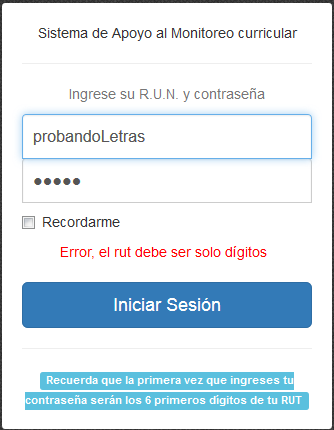
\includegraphics[width=0.5\textwidth]{images/Capitulo_5/REQF-01.png}
		\caption[REQF-01: Autentificación de usuario]{REQF-01: Autentificación de usuario \footnote{}}
		\label{REQF-01}
	\end{figure}
	\footnotetext{Elaboración propia.}
	
	
	Se realizaron distintas pruebas para comprobar el correcto funcionamiento de este requisito. A continuación se describen las distintas pruebas realizadas:
	\begin{itemize}
		\item Validación de números: El nick del usuario es su R.U.N. sin el dígito verificador, por lo que el sistema tiene que validar si el usuario ingresa cualquier carácter que no corresponda a un dígito. En caso de que el usuario ingrese algún carácter que no sea dígito, el sistema muestra el siguiente mensaje: \textbf{Error, el rut debe ser solo dígitos.}
		
		\item Validación nula: Los  dos campos solicitados  este formulario son campos obligatorios, por lo que si el usuario hace click en iniciar sesión y no ha completado estos campos, el sistema muestra un mensaje de alerta, impidiendo que el servidor realice cálculos innecesarios. Esta validación se ilustra en la Figura \ref{REQF-01-null}.
	\end{itemize}
	
	\begin{figure}[H]
		\centering
		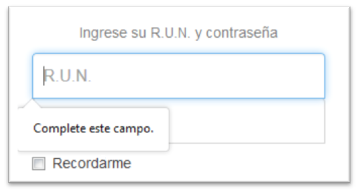
\includegraphics[width=0.7\textwidth]{images/Capitulo_5/REQF-01-null.png}
		\caption[REQF-01: Autentificación de usuario, validación de campos nulos]{REQF-01: Autentificación de usuario, validación de campos nulos}
		\label{REQF-01-null}
	\end{figure}
	
\subsection{REQF-02: Gestión de perfil}

\begin{figure}[H]
	\centering
	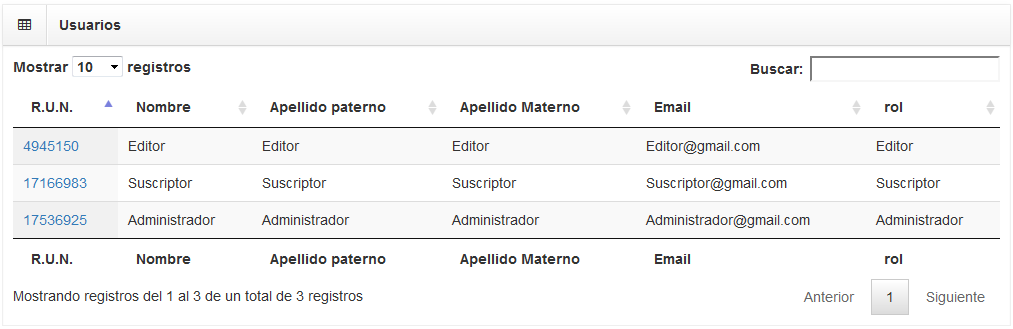
\includegraphics[width=1\textwidth]{images/Capitulo_5/REQF-02.png}
	\caption[REQF-02: Gestión de perfil]{REQF-02: Gestión de perfil}
	\label{REQF-02}
\end{figure}

La Figura \ref{REQF-02} ilustra la gestión de perfiles del sistema,  este requerimiento solo puede ser accedido por un usuario de tipo administrador.
\\
En primer lugar se realizaron pruebas para comprobar que los usuarios del tipo Editor y Suscriptor  no tuvieran acceso, para ello se crearon  tres usuarios con los tres tipos de perfiles existentes, con el fin de autentificarse y tratar de acceder a este requisito. los resultados muestran en la Tabla \ref{pruebas_gestionPerfiles}.

\newpage
	\begin{longtable}{l |l}
		
		\caption{Resultados de pruebas del acceso a la gestión de perfiles}
		\label{pruebas_gestionPerfiles}\\
		
		
		\hline
		\endfirsthead
		\multicolumn{2}{c}%
		{\tablename\ \thetable\ -- \textit{Continuación de la pagina anterior}} \\
		\hline
		
		\hline
		\endhead
		\hline \multicolumn{2}{r}{\textit{Continúa en la página siguiente}} \\
		\endfoot
		\hline
		\endlastfoot
		\rowcolor{LightBlue2} Tipo de perfil & Resultado de acceso\\ \hline
		
		Administrador & Se pudo acceder exitosamente.\\ \hline
		
		Editor & No se pudo acceder.\\ \hline
		
		Suscriptor & No se pudo acceder.\\ \hline \hline
	\end{longtable}

En segundo lugar se realizaron pruebas para las siguientes operaciones básicas de este requisito: Actualizar usuario y Eliminar usuario. el proceso y los resultados de cada prueba se detallan a continuación.

\mysubparagraph{Actualizar usuario}

Uno de los Errores encontrados al momento de validar esta acción, fue que al tratar de actualizar  un usuario en particular  los datos que se enviaban mediante la petición POST al servidor no eran los correctos. El error detectado se puede apreciar gráficamente en las Figuras \ref{REQF-02-actualizar} y \ref{REQF-02-post}.


\begin{figure}[H]
	\centering
	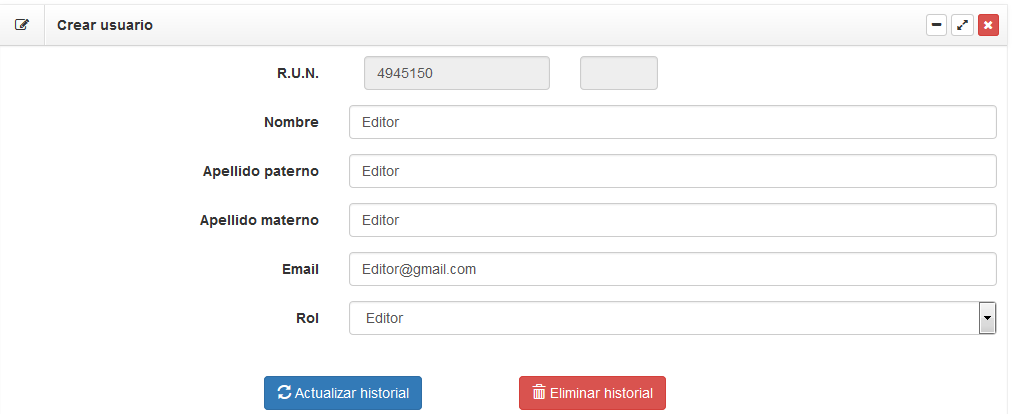
\includegraphics[width=1\textwidth]{images/Capitulo_5/REQF-02-agregar1.png}
	\caption[REQF-02: Gestión de perfil, Actualizar usuarios]{REQF-02: Gestión de perfil, Actualizar usuarios}
	\label{REQF-02-actualizar}
\end{figure}

Aunque el usuario autentificado esta intentando editar el  R.U.N. 4.945.150, en la Figura \ref{REQF-02-post}  se puede apreciar que, entre las variables que se están enviando, esta la variable Rut, que corresponde al R.U.N. editado, sin embargo el valor que esta tomando la variable  Rut no corresponde al R.U.N. editado, si no  que se esta enviando el R.U.N. de la persona autentificada. Este error fue corregido a tiempo.
\begin{figure}[H]
	\centering
	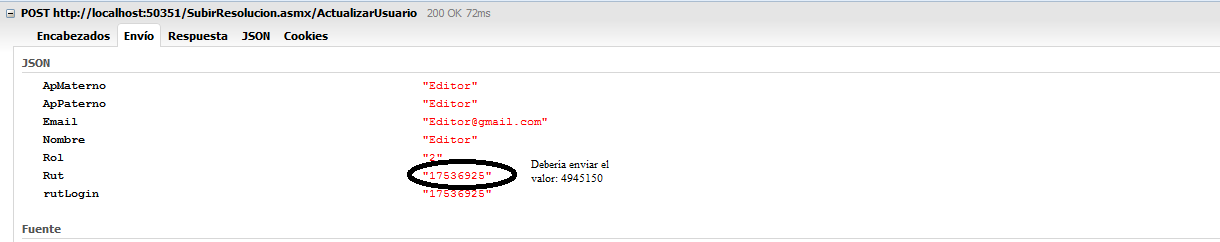
\includegraphics[width=1\textwidth]{images/Capitulo_5/REQF-02-post.png}
	\caption[REQF-02: Gestión de perfil, depuración de los datos enviados mediante la petición POST]{REQF-02: Gestión de perfi, depuración de los datos enviados mediante la petición POST}
	\label{REQF-02-post}
\end{figure}

\mysubparagraph{Eliminar usuario}

Comprobar el correcto funcionamiento del mensaje de alerta que se muestra en la Figura \ref{REQF-02-eliminar} era el principal objetivo de la validación de esta acción, ya que como se mencionó en la Sección \ref{Dificultades}, ASP.NET trabaja de una forma particular las peticiones POST de complementos externos.
\begin{figure}[H]
	\centering
	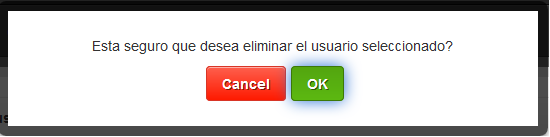
\includegraphics[width=1\textwidth]{images/Capitulo_5/REQF-02-Eliminar.png}
	\caption[REQF-02: Gestión de perfil, Mensaje de verificación para eliminar algún usuario]{REQF-02: Gestión de perfi, Mensaje de verificación para eliminar algún usuario}
	\label{REQF-02-eliminar}
\end{figure}

La verificación de esta acción se realizó mediante eliminaciones de registro. Se comprobó que los botones de la alerta generada(``Cancel'' y ``Ok'') realizaran sus respectivas acciones, además, se verificó de que si el registro eliminado poseía algún documento, éste fuera eliminado del servidor.


\subsection{REQF-03: Desplegar historial curricular}

Este requerimiento no necesitó mayores pruebas puesto que es un requerimiento de visualización.

\subsection{REQF-04: Registro de usuarios}

Uno de los datos que NO se pueden modificar una vez que se haya creado el usuario, es el R.U.N., por lo que es de vital importancia que este dato se ingrese correctamente al momento de registrar al usuario, para ello se consideró validar la existencia del R.U.N. ingresado mediante el plugins jQuery.Rut.js. \\

En caso de que el R.U.N. ingresado no existiera el sistema muestra gráficamente un mensaje de que el R.U.N. no existe (Ver Figura \ref{REQF-02-rut}), impidiendo que el usuario se almacene en la base de datos.

\begin{figure}[H]
	\centering
	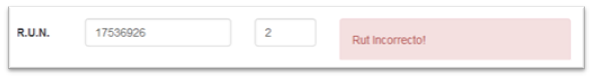
\includegraphics[width=1\textwidth]{images/Capitulo_5/REQF-02-rut.png}
	\caption[REQF-02: Gestión de perfil]{REQF-02: Gestión de perfil}
	\label{REQF-02-rut}
\end{figure}

Con respecto a los demás campos se validó que todos los campos sean obligatorios y que el formato del correo electrónico sea un formato  válido.


\subsection{REQF-05:Gestión de documentos}

Se realizaron distintas pruebas para comprobar el correcto funcionamiento de este requisito. A continuación se describen las distintas pruebas realizadas:
\begin{itemize}
	\item Validación nula: Todos los  campos solicitados en  este formulario son campos obligatorios, por lo que si el usuario deja un campo sin completar, y luego  hace click en Subir archivos, el sistema de forma inmediata marca en rojo todos los campos que no se han completado, y le informa al usuario de que son campos obligatorios.
	
	\item Validación de Formato de archivos: Se intentó subir archivos de distintos formatos (.jpg, word, ppt, etc) y el resultado que el sistema muestra un mensaje de Alerta indicando que el formato no es el correcto (Ver Figura \ref{REQF-05} ).
	
	\item Validación de eliminación de archivos: Se eliminaron registros curriculares con el fin de verificar que el registro se eliminara en su totalidad del sistema, es decir, que se eliminaran el registro en la base de dato y que se eliminara los archivos vinculados a ese registro eliminado del servidor.
\end{itemize}


\begin{figure}[H]
	\centering
	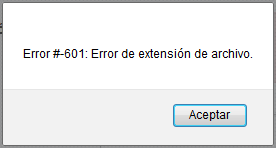
\includegraphics[width=0.5\textwidth]{images/Capitulo_5/REQF-05.png}
	\caption[REQF-05: Gestión de documentos, Mensaje de alerta ]{REQF-05: Gestión de documentos, Mensaje de alerta }
	\label{REQF-05}
\end{figure}
\subsection{REQF-06:Visor de PDF}

Este requerimiento no necesitó mayores pruebas puesto que es un requerimiento de visualización.

\subsection{REQF-07:Notificaciones}


Este requisito se validó en conjunto con los demás requisitos, ya que el sistema de notificaciones esta presente en todo el sistema.
\\

Básicamente el usuario se cercioró de que el sistema de alertas este presente cuando un usuario autentificado realizara alguna operación sobre los datos del sistema.
\\

 En la Figura \ref{REQF-07} se muestra un ejemplo de una notificación exitosa.
 
\begin{figure}[H]
	\centering
	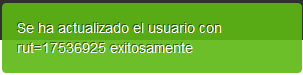
\includegraphics[width=0.5\textwidth]{images/Capitulo_5/REQF-07.png}
	\caption[REQF-07: Notificaciones, alerta exitosa ]{REQF-07: Notificaciones,alerta exitosa }
	\label{REQF-07}
\end{figure}

A  pesar de que el sistema de notificaciones esta presente en toda la plataforma, éste requisito fue casi uno de los últimos en ser programados, a causa de esto, hubieron muchas acciones que NO tenían su alerta activa.

\subsection{REQF-08:Almacenar bitácora de los usuarios}


El objetivo de este requisito es facilitar la identificación  de la localización de los errores del sistema, por lo que es de vital importancia su correcto funcionamiento.\\

La validación de este requerimiento es muy distinta a todas las otras validaciones, ya que las validaciones anteriores dependían de los mensajes de alerta que el sistema entregaba, mientras que la validación de este requerimiento depende estrictamente de las salidas de los procedimientos almacenados de la base de datos y de las salidas de los servicios web del sistema, a causa de esto, el alumno tesista se enfocó en validar  los procedimientos y los servicios web. Las distintas pruebas realizadas se describirán a continuación.
\\

En primer lugar, el alumno tuvo que validar que las salidas de todos los procedimientos sean estándar, puesto que las salidas se almacenan en la tabla REGISTRO, y esta tabla posee  campos obligatorios. El proceso de validación se realizó mediante la ejecución de los procedimientos almacenados y la lectura de las salidas de estos mismos en la consola de SQL Server. Los campos de las salidas de los procedimientos que producen cambios en el sistema son los siguientes:


\begin{itemize}
	\item \textbf{ErrorNumber:} Identificador único del mensaje.
	\item \textbf{ErrorMessage:} Descripción del mensaje.
	\item \textbf{ErrorDate:} Fecha en la que ocurrió en evento.
\end{itemize}

Una vez  validados los procedimientos, se procedió  a validar los servicios web, para ello fue de gran ayuda el complemento Firebug, ya que el Alumno validó las salidas de los servicios, mediante textos enviados  a la consola de Firebug. En la Figura \ref{REQF-09}, se puede apreciar una salida de un mensaje de error de un servicio web.

\begin{figure}[H]
	\centering
	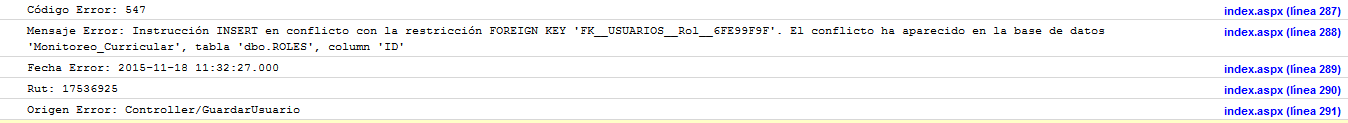
\includegraphics[width=1\textwidth]{images/Capitulo_5/REQF-09.png}
	\caption[REQF-09: Almacenar bitácora de los usuarios, salida de un procedimiento. ]{REQF-07: Almacenar bitácora de los usuarios, salida de un procedimiento. }
	\label{REQF-09}
\end{figure}
\subsection{REQF-09:Visualización de bitácora}

Este requerimiento no necesitó mayores pruebas puesto que es un requerimiento de visualización.